% **************************************************************************************************************
% A Classic Thesis Style
% An Homage to The Elements of Typographic Style
%
% Copyright (C) 2018 André Miede and Ivo Pletikosić
%
% If you like the style then I would appreciate a postcard. My address
% can be found in the file ClassicThesis.pdf. A collection of the
% postcards I received so far is available online at
% http://postcards.miede.de
%
% License:
% This program is free software; you can redistribute it and/or modify
% it under the terms of the GNU General Public License as published by
% the Free Software Foundation; either version 2 of the License, or
% (at your option) any later version.
%
% This program is distributed in the hope that it will be useful,
% but WITHOUT ANY WARRANTY; without even the implied warranty of
% MERCHANTABILITY or FITNESS FOR A PARTICULAR PURPOSE.  See the
% GNU General Public License for more details.
%
% You should have received a copy of the GNU General Public License
% along with this program; see the file COPYING.  If not, write to
% the Free Software Foundation, Inc., 59 Temple Place - Suite 330,
% Boston, MA 02111-1307, USA.
%
% PLEASE SEE ALSO THE AUTHORS' NOTE REGARDING THIS LICENSE
% IN THE DOCUMENTATION (ClassicThesis.pdf --> Chapter 1 / Chapter01.tex)
% **************************************************************************************************************
\RequirePackage{silence} % :-\
    \WarningFilter{scrreprt}{Usage of package `titlesec'}
    %\WarningFilter{scrreprt}{Activating an ugly workaround}
    \WarningFilter{titlesec}{Non standard sectioning command detected}
\documentclass[ twoside,openright,titlepage,numbers=noenddot,%1headlines,
                headinclude,footinclude,cleardoublepage=empty,abstract=on,
                BCOR=5mm,paper=a4,fontsize=11pt,
		dvipsnames
                ]{scrreprt}

%********************************************************************
% Note: Make all your adjustments in here
%*******************************************************
\input{classicthesis-config}

%********************************************************************
% Bibliographies
%*******************************************************
\addbibresource{Bibliography.bib}
\addbibresource[label=ownpubs]{Eigene.bib}

%********************************************************************
% Hyphenation
%*******************************************************
%\hyphenation{put special hyphenation here}

% ********************************************************************
% GO!GO!GO! MOVE IT!
%*******************************************************
\begin{document}
\frenchspacing
\raggedbottom
\selectlanguage{american} % american ngerman
%\renewcommand*{\bibname}{new name}
%\setbibpreamble{}
\pagenumbering{roman}
\pagestyle{plain}
%********************************************************************
% Frontmatter
%*******************************************************
%*******************************************************
% Little Dirty Titlepage
%*******************************************************
\thispagestyle{empty}
%\pdfbookmark[1]{Titel}{title}
%*******************************************************
\begin{changemargin}{0mm}{-2cm}
\begin{center}
	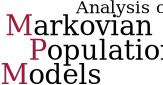
\includegraphics[width=0.7\textwidth]{gfx/titlepage.pdf}\\
	\bigskip
	\textsc{\myName}
    %\spacedlowsmallcaps{\myName} \\ \medskip

%   \begingroup
%       \color{CTtitle}\spacedallcaps{Analysis~of~Markovian~Population~Models}
%   \endgroup
\end{center}
\end{changemargin}

\include{FrontBackmatter/Titlepage}
\thispagestyle{empty}

\hfill
\vfill

{\raggedright
\noindent
Tag des Kolloqiums:  \\
Dekan:   \\  
Berichterstatter:  \myProf, \myOtherProf \\
Vorsitzender:  \\
Akademischer Mitarbeiter: \\
%\noindent
%\begin{tabular}{ r | l}
% Tag des Kolloqiums: & \\
% Dekan: &  \\  
% Berichterstatter: & \myProf \\    
%  & \myOtherProf \\
% Vorsitzender: & \\
%	Akademischer Mitarbeiter:
%\end{tabular}
\bigskip
\noindent
This dissertation was typeset in \LaTeX{}  using a design based on \texttt{\classicthesis}.
Hermann Zapf's \emph{Palatino} (\emph{\acsfont{URW} Palladio)}, \emph{Euler} and \emph{Optima} (\acsfont{URW} Classico) type faces are used.\\
\bigskip
\noindent
{Final version} as of \today.\\
\bigskip
\noindent
\textcopyright\ \myName, \myTime
}

%\cleardoublepage\include{FrontBackmatter/Dedication}
%\cleardoublepage\include{FrontBackmatter/Foreword}
\cleardoublepage\include{FrontBackmatter/Declaration}
\cleardoublepage%*******************************************************
% Abstract
%*******************************************************
%\renewcommand{\abstractname}{Abstract}
\pdfbookmark[1]{Abstract}{Abstract}
% \addcontentsline{toc}{chapter}{\tocEntry{Abstract}}
% \begingroup
% \let\clearpage\relax
% \let\cleardoublepage\relax
% \let\cleardoublepage\relax

\chapter*{Abstract}
We use moment properties to provide bounds on mean first-passage times and to improve statistical estimation of different quantities.  In particular, we use the variance reduction technique of \emph{linear control variates} in connection with these moment constraints.  We present a state-space lumping scheme that aggregates states in a grid structure.  Approximations based on this lumping are used to iteratively refine relevant and truncate irrelevant parts of the state-space.  This way, the algorithm learns a well-justified finite-state projection for different scenarios.  Existing Foster-Lyapunov functions often give sets that are far larger necessary for a given probability bound.  Here, we explore the possibility to improve upon such a function by \emph{local} alterations.  This leaves the global properties --~and thereby its guarantees~-- intact, while we obtain much tighter sets for the same probability bounds.

\cleardoublepage

\begin{otherlanguage}{ngerman}
\pdfbookmark[1]{Zusammenfassung}{Zusammenfassung}
\chapter*{Zusammenfassung}
Kurze Zusammenfassung des Inhaltes in deutscher Sprache\dots
\end{otherlanguage}

% \endgroup

\vfill

%\cleardoublepage\include{FrontBackmatter/Publications}
% \cleardoublepage%*******************************************************
% Acknowledgments
%*******************************************************
\pdfbookmark[1]{Acknowledgments}{acknowledgments}


% \begin{flushright}{\slshape
% 	The world of modelling can be hard; just as cruel as it is glamorous.}\\\medskip
% --- Cindy Margolis
% \end{flushright}


\vspace{3cm}

\begingroup
\let\clearpage\relax
\let\cleardoublepage\relax
\let\cleardoublepage\relax
\chapter*{Acknowledgments}
First of all I would like to thank my supervisors Verena Wolf and Luca Bortolussi both for introducing me into the fascinating topic of Markovian population models as well as giving me the freedom to explore topics and ideas.
I am also particularly grateful to my colleague Gerrit Großmann for the frequent stimulating discussions and collaborations.
Furthermore, I thank my coauthors Adish Singla, Felix Scherzinger, Jonas Klesen, and Julian Zimmerlin for the good discussions.

%\begin{itemize}
    %\item Verena, Luca
    %\item Gerrit
    %\item Thilo, Charalampos, Alex L, Timo, Joschka
    %\item other co-authors: 
    %\item \acsfont{DFG} and \acsfont{MULTIMODE}
    %\item family \& friends
%\end{itemize}


\endgroup

\cleardoublepage\include{FrontBackmatter/Contents}
%********************************************************************
% Mainmatter
%*******************************************************
\cleardoublepage
\pagestyle{scrheadings}
\pagenumbering{arabic}
%\setcounter{page}{90}
% use \cleardoublepage here to avoid problems with pdfbookmark
\part{Preliminaries}
\cleardoublepage\chapter{Introduction}
%\begin{center}
 %Machines were mice and men were lions\\
    %once upon a time.\\
    %But now that it's the opposite\\
    %it's twice upon a time.\\
    %\medskip
        %\emph{--- Moondog}
%\end{center}


The scientific method revolves around the evolution of falsifiable hypotheses.
Such hypotheses can be simple statements such as water being liquid at room temperature and an average air pressure.
All hypotheses involve some sort of model~--~some more well-defined than others.
In the natural sciences, we often deal with concentrations of different ``things''.
This could be the amount of some substance in a beaker or the number of agents waiting for some service.



Modelling often is a delicate balance of adequate representation and abstraction.
The former is the goal to capture all the relevant behaviours and effects in a model.
Abstractions are made for the benefit of both, explainability and facilitating analysis.

Simplify representation for more efficiency per computation.


% MFPT bounds

\Acfp{MPM} provide a
widely used framework to capture stochastic interactions between groups of identical agents.
This subclass of \acfp{CTMC}  is used
to describe the stochastic dynamics of systems in various domains.
Prominent applications are chemical reaction networks in quantitative
biology~\parencite{BuchWolkenhauer},
epidemic spreading~\parencite{porter2016dynamical}, performance analysis  of technical and
information systems~\parencite{bortolussi2013continuous,gast2019} as well as the behavior of
collective adaptive systems~\parencite{bernardo2016}.

% Stationary aggregation

In many areas of science, stochastic models  of interacting populations can describe systems in which the discrete population sizes evolve stochastically in continuous time.
Such problems naturally occur in a wide range of areas such as chemistry~\parencite{gillespie1977exact}, systems biology~\parencite{wilkinson2018stochastic,BuchWolkenhauer}, epidemiology~\parencite{mode2000stochastic} as well as    queuing systems~\parencite{breuer2003markov} and finance~\parencite{pardoux2008markov}.

Interactions between agents, commonly referred to as \emph{reactions}, happen at exponentially distributed random times. 
Their rate depends on the current system state, i.e.\ the population sizes.
This results in a continuous-time Markov chain semantics~\parencite{anderson2012continuous}.

% Bridging

\Acp{MPM} are widely used to model the time evolution of complex 
discrete phenomena in continuous time. Such problems naturally occur in a wide range of areas such as chemistry~\parencite{gillespie1977exact}, systems biology~\parencite{wilkinson2018stochastic,BuchWolkenhauer}, epidemiology~\parencite{mode2000stochastic} as well as    queuing systems~\parencite{breuer2003markov} and finance~\parencite{pardoux2008markov}.
% The Markov property renders model analysis   feasible but requires a complete description of the current state
% to describe the future behavior of the chain.
In many applications, an \ac{MPM} describes the stochastic interaction of populations of agents.
%and therefore exhibits a population structure.
The state variables are counts of individual entities of different populations.

% LCVs

Markovian Population Models that are used to describe cellular processes are often subject to inherent stochasticity.
The dynamics of gene expression, for instance, is influenced by 
single random events (e.g.\ transcription factor binding) and 
hence, models that take this randomness into account must monitor
discrete molecular counts and reaction events that change these counts.
Discrete-state continuous-time Markov chains have successfully  been
used to describe  networks of chemical reactions
over time that correspond to the basic events of such processes. 
The time-evolution of the corresponding probability distribution is 
given by the chemical master equation, whose numerical solution is
extremely challenging because of the enormous size of the underlying
state-space. 

\section{Organization}
All contributions presented in this thesis are related to \aclp{MPM}.
Therefore the background chapter, i.e.\ \autoref{ch:background} is relevant
to all later parts of the thesis.
The prerequisite for \autoref{ch:statagg} and \autoref{ch:bridging} is the aggregation
technique presented in \autoref{ch:lumping}.
Note that \autoref{ch:MFPT} and \autoref{ch:cvinsrns} share the temporal moment approach presented
in both chapters.
\autoref{fig:chap_deps} provides an overview of the dependencies between chapters.
\begin{figure}[htb]
	\centering
\begin{tikzpicture}
	\begin{scope}
  \path[mindmap,concept color=gray!25,text=black,level 1 concept/.append style =
      {sibling angle=40}]
        node[concept] {\autoref{ch:background}\\Markovian\\population\\models}
    [clockwise from=-30]
        child[concept]{
            node[concept] (lya) {\autoref{ch:lyapunov}\\Lyapunov functions}
        }
    child[concept] {
	    node[concept] {\autoref{ch:lumping}\\Aggregation}
	    [clockwise from=-15]
	    child[concept] {
            node[concept] (stat) {\autoref{ch:statagg}\\Stationary behavior}
	    }
	    child[concept] {
		    node[concept] {\autoref{ch:bridging}\\Bridging problem}
	    }
	    child[concept] {
		    node[concept] {\autoref{ch:is}\\Importance Sampling}
	    }
    }
    child[concept] {
	    node[concept] (cv) {\autoref{ch:cvinsrns}\\Control variates}
    }
    child[concept] {
	    node[concept] (mfpt) {\autoref{ch:MFPT}\\Bounding \acsfont{MFPT}s}
    }
    ;
    \begin{pgfonlayer}{background}
        \draw [concept connection] (cv) edge (mfpt);
        \draw [concept connection] (lya) edge (stat);
    \end{pgfonlayer}
	\end{scope}
 %    \begin{pgfonlayer}{background}
 %  %\draw [draw=gray!25,fill=gray!25, decorate,decoration=circle connection bar]
 %            \path (cv) to[draw=gray!25,color=gray!25,fill=gray!25, circle connection bar] (mfpt);
%%     \draw[circle connection bar]
%%%%% (cv) edge (mfpt);
 %    \end{pgfonlayer}
\end{tikzpicture}
	\caption{\label{fig:chap_deps}Chapter dependencies.}
\end{figure}


%*******************************************************
% Publications
%*******************************************************
\section{Previous Publications}%\graffito{This is just an early --~and currently ugly~-- test!}
The ideas and much of the presented results have appeared previously in the following publications.
As such, the content of most chapters have undergone peer-review and been published in various conference proceedings.
The publications and their respective sections are as indicated below.

\begin{itemize}

\item \autoref{ch:MFPT} has with minor differences been published as
\begin{quote}
    \fullcite{backenkohler2019bounding}.
\end{quote}
The approach was conceived by M.\ B.
Author M.\ B.\ performed the implementation and evaluation with feedback from the other authors.
All authors contributed to the text.

\item \autoref{ch:cvinsrns} has with minor differences been published as
\begin{quote}
    \fullcite{backenkohler2019control}.
\end{quote}
The control variate approach was conceived by M.\ B.\ and V.\ W. The refinement algorithm was developed during discussions of all authors.
Author M.\ B.\ performed the implementation and evaluation with feedback from the other authors.
All authors contributed to the text.

The contents of \autoref{sec:splitting} have been published in the article
\begin{quote}
    \fullcite{backenkohler2021variance}.
\end{quote}
The control variate approach was conceived by M.\ B.\ and V.\ W. The resampling algorithm was developed during discussions of all authors.
Author M.\ B.\ performed the implementation and evaluation with feedback from the other authors.
All authors contributed to the text.

\item \autoref{ch:statagg} has with minor differences been published as
\begin{quote}
    \fullcite{backenkohler2021abstraction}.
\end{quote}
The lumping approach was conceived by M.\ B.
All authors contributed to the text.

\item \autoref{ch:bridging} has with minor differences been published as
\begin{quote}
    \fullcite{backenkohler2020analysis}.
\end{quote}
\end{itemize}
The lumping approach was conceived by M.\ B.
All authors contributed to the text.
\autoref{ch:lumping} is in large part based on this and the latter two publication above.
\autoref{ch:background} contains introductory material and examples from all of the above publications.

%\noindent Put your publications from the thesis here. The packages \texttt{multibib} or \texttt{bibtopic} etc. can be used to handle multiple different bibliographies in your document.

% \begin{refsection}[ownpubs]
%     \small
%     \noparencite{*} % is local to to the enclosing refsection
% 
%     \printbibliography[heading=none]
% \end{refsection}



\cleardoublepage\chapter{Background}

\section{Continuous-time Markov Chains}
\begin{itemize}
   \item Basic definitions
   \item Properties (non-explosivity, ergodicity, reversibility, irreducibility etc.)
\end{itemize}

\section{Markovian Population Models}
A Markov population model (MPM)
describes the stochastic interactions
among agents of distinct types in a well-stirred system.
This assumes that all agents are equally distributed in space, which
allows us to keep track only of the overall copy number of agents for each type.
Therefore the state-space is $\mathcal{S}\subseteq\mathbb{N}^{n_S}$ where
$n_S$ denotes the number of agent types or populations.
Interactions between agents are expressed as \emph{reactions}.
These reactions have associated
gains and losses of agents, given by non-negative integer vectors   
${v}_j^{-}$ and ${v}_j^{+}$ for reaction $j$, respectively. The overall change by a reaction is given by the vector $v_j = v_j^+ - v_j^-$.
A reaction between agents of types $S_1,\dots, S_{n_S}$ is specified in the following form:
\begin{equation}\label{eq:reaction}
    \sum_{\ell=1}^{n_S} v_{j\ell}^{-} S_\ell
    \xrightarrow{\alpha_j( x)}
    \sum_{\ell=1}^{n_S} v_{j\ell}^{+} S_\ell\,.
\end{equation}
The propensity function $\alpha_j$ gives the rate of the exponentially distributed firing
time of the reaction as a function of the current system state $x\in \mathcal{S}$.
In population models, \emph{mass-action} propensities are most common.
In this case the firing rate is given by the product of the number
of reactant combinations in $x$ and a
\emph{rate constant} $c_j$, i.e.
\begin{equation}\label{eq:stoch_mass_action}
    \alpha_j({x})\coloneqq c_j\prod_{\ell=1}^{n_S}\binom{x_\ell}{v_{j\ell}^{-}}\,.
\end{equation}
In this case, we give the rate constant in \eqref{eq:reaction} instead of the function $\alpha_j$.
For a given set of $n_R$ reactions, we define a stochastic
process $\{{{X}}_t\}_{t\geq 0}$ describing the evolution of the population
sizes over time $t$.
Due to the assumption of exponentially distributed firing times\marginpar{Note that in addition mild regularity assumptions
are   necessary for the existence of a unique CTMC $X$, such as non-explosiveness \cite{anderson2012continuous}.
These assumptions  are  typically
valid for realistic reaction networks.},  $ X$ is
a continuous-time
Markov chain (CTMC) on $\mathcal{S}$ with infinitesimal  generator matrix $Q$, where
the entries of $Q$ are
\begin{equation}\label{eq:cme_generator}
    Q_{ x,  y} = \begin{cases}
        \sum_{j: x+ v_j = y}\alpha_j( x)\,,&\text{if}\; x\neq
         y,\\[1ex]
        -\sum_{j=1}^{n_R} \alpha_j( x)\,, &\text{otherwise.}
    \end{cases}
\end{equation}
The probability distribution over time is given by an
initial value problem.
Given an initial state $x_0$, the distribution\marginpar{We assume an enumeration of all states in  $\mathcal{S}$. We simply write $x_i$ for the state with index $i$ and drop this notation for entries of a state $x$.  }
\begin{equation}\label{eq:forw_prob}
\pi(x_i, t)=\Pr(X_t=x_i\mid X_0=x_0),\quad t\geq 0
\end{equation}
evolves according to the Kolmogorov forward equation
\begin{equation}\label{eq:forward}
\frac{d}{dt}\pi(t) = \pi(t) Q\,,
\end{equation}
where $\pi(t)$ is an arbitrary vectorization $(\pi(x_1,t), \pi(x_2,t),\dots,\pi(x_{|\mathcal{S}|},t))$ of the states.
\eqref{eq:forw_prob} given for a single state, in the context of quantitative biology, it is commonly referred to
as the \emph{chemical master equation} (CME)
\begin{equation}\label{eq:cme}
    \frac{d\pi}{d t} ( x,t) =
    \sum_{j=1}^{n_R}\left(
        \alpha_j( x- v_j)\pi( x- v_j,t) - \alpha_j( x)\pi( x,t)
    \right)\,.
\end{equation}
A direct solution of \eqref{eq:cme} is usually not possible.
If the state-space with non-negligible probability is suitably small, a state space
truncation could be performed. That is, \eqref{eq:cme} is integrated on a possibly time-dependent subset
$\hat{\mathcal{S}}_t\subseteq\mathcal{S}$ \cite{henzinger2009sliding,munsky2006finite,spieler2014numerical}.
Instead of directly analyzing \eqref{eq:cme}, one often resorts to simulating trajectories.
A trajectory $\tau=x_0t_1x_1t_1\dots t_n x_n$ over the interval $[0,T]$ is a sequence of states $x_i$
% \vw{warum s nicht x fuer states? Eigentlich i=0 }
and corresponding
jump times $t_i$, $i=1,\dots,n$ and $t_n=T$.
We can sample trajectories of $X$ by using stochastic simulation~\cite{gillespie1977exact}.

\paragraph{Example} Consider a birth-death process as a simple example. This model is used to describe a wide variety of phenomena and often constitutes a sub-module of larger models.
For example, it represents an M/M/1 queue with service rates being linearly dependent on the queue length.
Note that even for this simple model, the state-space is countably infinite.
% \MB{could remove model environment for space}
\begin{model}[Birth-Death Process]\label{model:bd}
The model consists of exponentially distributed arrivals and service times proportional to queue length. It can be expressed using two mass-action reactions:
$$ \varnothing \xrightarrow{\mu} S \qquad\text{and}\qquad S \xrightarrow{\gamma} \varnothing\,.$$
The initial condition $X_0=0$ holds with probability one.
\end{model}

For \autoref{model:bd} the change of probability mass in a single state $x>0$ is described by expanding
\eqref{eq:cme} and
$$\frac{d}{dt}\pi_t(x)=\gamma \pi_t(x-1) + \delta \pi_t(x+1) - (\gamma + \delta)\pi_t(x)\,.$$

\section{Stochastic Simulations}
We can generate trajectories of this model by choosing either reaction, with a probability that is
proportional to its rate given the current state $x_i$ \cite{gillespie1977exact}.
The jump time $t_i- t_{i+1}$ is determined by sampling from an exponential distribution with rate $\gamma+x_i\delta$.
The simulation algorithm consists of repeatedly evaluating the race condition and jump times induced by~\eqref{eq:cme_generator}.
\begin{algorithm}
    $\tau \leftarrow$ empty list, $s\leftarrow$ sample from $\pi_0$, $t\leftarrow 0$\;
    \While{$t<T$}{
        $r_i\leftarrow\alpha_i(s),\;i=1,\dots,n_R$\;
	$k\leftarrow$ sample reaction $i$ with probability $r_i/\sum_ir_i$\;
	$dt\sim \text{Exp}\left(\sum_i r_i\right)$\;
        $s\leftarrow s + v_k$\;
	$t \leftarrow t + dt$\;
    }
    \textbf{return} $\tau$\;
    \caption{\label{alg:ssa}Sample a trajectory}
\end{algorithm}


\section{Moment Dynamics}

\ctparttext{
	We use moment properties
	to bound mean first-passage times and
	to improve statistical estimation of different quantities.
%%%%%%  In particular, we use the variance reduction technique
%%%%%%  of \emph{linear control variates} in connection with these moment
%%%%%%  constraints.
}
\part{Moment-Based Methods}
\cleardoublepage\include{Chapters/MFPT}
\cleardoublepage\chapter{Linear Control Variates for Monte~Carlo \mbox{Estimation}}\label{ch:cvinsrns}
% \author{Michael Backenk\"ohler\inst{1}, Luca Bortolussi\inst{1,2}, Verena Wolf\inst{1}}
% \authorrunning{M.\ Backenk\"ohler et al.}
% \institute{\inst{1}Saarland University, Germany, \inst{2}University of Trieste, Italy}
% \maketitle
% \begin{abstract}
% Stochastic simulation is a widely used method for 
% estimating quantities in models of chemical 
% reaction networks where uncertainty plays a crucial role.
% However,  reducing  the statistical uncertainty of the corresponding  
% estimators requires the generation of a large number 
% of simulation runs, which is computationally expensive.
% To reduce the number of necessary runs, we propose a
% variance reduction technique based on control variates.
% We exploit  constraints on the statistical moments of the 
% stochastic process
% to reduce the estimators' variances.
% We develop an algorithm that selects appropriate control
% variates in an on-line fashion and demonstrate the efficiency of our approach  on several case studies.
% 
% \keywords{Chemical Reaction Network  \and Chemical Master Equation \and Stochastic Simulation Algorithm
% \and Moment Equations \and Control Variates \and Variance Reduction}
% \end{abstract}
% %
% %
%\section{Introduction}

Analysis approaches based on sampling, such as the \acf{SSA}~\parencite{gillespie1977exact}\turnto{sec:ssa}, can  be applied
independent of the size of the model's state-space. 
However, statistical approaches are costly since a large number
of simulation runs is necessary to reduce the statistical 
inaccuracy of estimators. This problem is particularly severe
if reactions occur on multiple time scales or if the event of interest is rare.
A particularly popular technique to speed up simulations is $\tau$-leaping which applies
multiple reactions in one step of the simulation.
However, such multi-step simulations rely on certain assumptions about
the number of reactions in a certain time interval. These assumptions
are typically only approximately fulfilled and therefore introduce  approximation
errors on top of the statistical uncertainty of the considered point estimators.

Moment-based techniques offer a fast approximation of the statistical moments of the model. 
The exact moment dynamics can be expressed as an infinite-dimensional system of \acp{ODE}, which cannot be directly  integrated for a transient analysis.
Hence, ad-hoc approximations need to be introduced, expressing higher order moments as functions of lower-order ones \parencite{ale2013general,engblom2006computing}.
However, moment-based approaches rely on assumptions about the dynamics that are
often not even approximately fulfilled and may lead to high approximation errors. 
Recently, equations expressing the moment dynamics have also been used as constraints for parameter
estimation \parencite{backenkohler2018moment} and for computing moment bounds using semi-definite programming \parencite{dowdy2018dynamic,ghusinga2017exact}.

In this work, we propose a combination of such moment constraints with the \ac{SSA} approach.
Specifically, we   interpret these constraints as random variables 
that are correlated with the estimators of interest usually given as functions of chemical population variables.
These constraints can be used  as  (linear) \acfp{CV} in order to improve the final estimate and reduce its variance \parencite{lavenberg1982statistical,szechtman2003control}.
The method is easy on an intuitive level: If a control variate
is positively correlated with the function to be estimated then 
we can use the estimate of the variate to
adjust the target estimate.
%more details

The incorporation of control variates into the \ac{SSA}
introduces   additional simulation costs for the calculation of the constraint values.
These values are integrals over time, which we accumulate  based on the
piece-wise constant trajectories.
This introduces a trade-off between the variance reduction that is achieved
by using control variates versus the increased simulation cost.
This trade-off is expressed as the product of the variance reduction ratio
and the cost increase ratio.

For a good trade-off, it is crucial to find an appropriate set of control variates.
Here we propose a class of constraints which is parameterized by a moment vector
and a weighting parameter, resulting in infinitely many choices.
We present an algorithm that samples from the set of all constraints and
proceeds to remove constraints that are either only weakly correlated with the
target function or are redundant in combination with other constraints.

In a case study, we explore different variants of this algorithm
both in terms of generating the initial constraint set and of
removing  weak or redundant constraints.
We find that the algorithm's efficiency is superior to a standard estimation procedure
using stochastic simulation alone
in almost all cases.

Although in this work we focus on  estimating first order moments at
fixed time points, the proposed approach can in principle deal with any property that can
be expressed in terms of expected values such as probabilities
of complex path properties.
Another advantage of our technique is that an increased efficiency is achieved without the price of an additional approximation error as it is the case for methods based on moment approximations or multi-step simulations.

\section{Related Work}\label{sec:cv:related}
\paragraph{State-space Truncations}
If the state-space is finite and small enough one can deal with the underlying Markov
chain directly.
But there are also  cases where the transient distribution has an infinitely large support
and one can still deal with explicit state probabilities.
To this end, one can fix a finite state-space, that should contain most of the
probability~\parencite{munsky2006finite}. Refinements of the method work
dynamically and adjust the state-space according to the transient
distributions~\parencite{andreychenko2011parameter,henzinger2009sliding,mateescu2010fast}.

\paragraph{Moment Approximations}
On the other end of the spectrum there are mean-field approximations, 
which model the mean densities faithfully in the system size limit~\parencite{bortolussi2013continuous}.
In between there are techniques such as moment closure \parencite{singh2006lognormal}, that
not only consider the mean, but also the variance and other higher order moments.
These methods depend on ad-hoc approximations of higher order moments to
close the \ac{ODE} system given by the moment equations.
Yet another class of methods approximate molecular counts continuously and approximate the dynamics in such a continuous space, e.g. the system size expansion~\parencite{van1992stochastic} and the
chemical Langevin equation~\parencite{gillespie2000chemical}.

While the moment closure method uses ad-hoc approximations for high order moments to
facilitate numerical integration, they can be avoided in some contexts.
For the equilibrium distribution, for example, the time-derivative of all moments is equal to zero.
This directly yields constraints that have been used for parameter estimation at
steady-state~\parencite{backenkohler2018moment}
and bounding moments of the equilibrium distribution using semi-definite
programming~\parencite{ghusinga2017estimating,ghusinga2017exact,kuntz2017rigorous}.
The latter technique of bounding moments has been successfully adapted in the 
context of transient analysis~\parencite{dowdy2018dynamic,sakurai2017convex,sakurai2019bounding}.
We adapt the constraints proposed in these works to improve statistical estimations via stochastic
simulation (cf.\ \autoref{sec:cv:moments}).


\paragraph{Monte Carlo Simulation}
While the above techniques give a deterministic output, stochastic simulation generates
single executions of the stochastic process~\parencite{gillespie1977exact}.
This necessitates accumulating large numbers of simulation runs to estimate
quantities.
This adds a significant computational burden. Consequently, considerable effort
has been directed at lowering this cost.
A prominent technique is $\tau$-leaping~\parencite{gillespie2001approximate},
which in one step performs multiple instead of only a single reaction.
Another approach is to find approximations that are specific to the problem at hand,
such as approximations based on time-scale separations~\parencite{cao2005slow,bortolussi2015efficient}.

Recently, multilevel Monte Carlo methods have been applied in to time-inhomogenous
\ac{MPM}~\parencite{anderson2018low}. In this techniques estimates are combined
using estimates of different approximation levels.

% \parencite{goodman2009coupling}

The most prominent application of a variance reduction technique in the context
of stochastic reaction networks is importance sampling~\parencite{kuwahara2008efficient}.
This technique relies on an alteration of the process and then weighting samples
using the likelihood-ratio between the original and the altered process.
% \vw{This sentence stands here a bit lonely. Maybe shortly explain importance sampling? Also: there are papers about importance splitting (does this count as variance reduction technique? I would guess so.)}
% 

% \vw{Warum sagst Du hier nicht kurz etwas über numerische Lösungen der CME und die Schwierigkeiten? Eigentlich wäre numerische Lösung vorzuziehen wenn sie nicht so schwierig wäre}




\section{Moment Constraints}\label{sec:cv:moments}
The time-evolution of $\E{f(X_t)}$ for some function $f$ is given by \eqref{eq:mom_ode}\turnto{eq:mom_ode}.
The integration of \eqref{eq:mom_ode} with such functions $f$ is well-known in the context of
moment approximations of \ac{MPM}.
For most models the arising \ac{ODE} system is infinitely large, because the time-derivative of
low order moments usually depends on the values of higher order moments.
To close this system, \emph{moment closures}, i.e.\ ad-hoc approximations of higher order moments
are applied \parencite{schnoerr2015}.
The main drawback of this kind of analysis is that it is not known whether the chosen closure gives
an accurate approximation for the case at hand.
Here, such approximations are not necessary, since we will apply the moment dynamics in the context
of stochastic sampling instead of trying to integrate \eqref{eq:mom_ode}.

Apart from integration strategies,
setting \eqref{eq:mom_ode} to zero has been used as a constraint for parameter estimation at steady-state
\parencite{backenkohler2018moment} and bounding moments at steady-state~\parencite{dowdy2018bounds,ghusinga2017exact,kuntz2017rigorous}.
The extension of the latter has recently lead to the adaption of these constraints
to a transient setting~\parencite{dowdy2018dynamic,sakurai2019bounding}.
These two transient constraint variants are analogously derived by multiplying \eqref{eq:mom_ode}
by a time-dependent, differentiable weighting function $w(t)$ and integrating:

As in the previous chapter,\turnto{eq:exp_constraint} multiplication with $w(t)$ and integration on $[t_0, T]$ yields~\parencite{dowdy2018dynamic,sakurai2019bounding}
\begin{multline}\label{eq:poly_con}
        w(T)\E{f(X_{T})}
        - w(t_0)\E{f(X_{t_0})}
	- \int_{t_0}^{T}\frac{dw(t)}{dt}\E{f(X_t)}\,dt\\
        =\sum_{j=1}^{n_R}\int_{t_0}^{T}w(t)
        \E{\left(f{(X_t + v_j)} - f(X_t)\right)\alpha_j(X_t)}\,dt
\end{multline}
While many choices of $f$ are possible, for this work we will restrict ourselves to
monomial functions $f(x)=x^m$, $m\in\mathbb{N}^{n_S}$
% \vw{ich dachte, m soll ein Vektor sein}
i.e.\ the \emph{non-central} or \emph{raw moments} of the process.
In the context of computing moment bounds via semi-definite programming
the polynomial $w(t)=t^s$~\parencite{sakurai2019bounding} and the exponential $w(t)=e^{\lambda(T - t)}$~\parencite{dowdy2018dynamic}
have been proposed.
While both choices proved to be effective in different case studies, relying solely on the latter choice,
\marginpar{In \autoref{ch:MFPT} we chose the monomial, such that \eqref{eq:poly_con} would admit the interpretation of temporal moments. Here the exponential is a good choice, because it can model both increasing and decreasing weighting.}
i.e.\ \[
	w(t)=e^{\lambda(T - t)} \] was sufficient.

% Let $$
% % \hat m^{(s)}_f = \int_{t_0}^{T}t^s\E{f(X_t)}\,dt
% % \quad\text{and}\quad
%  {m}^{(\lambda)}_f = \int_{t_0}^{T}e^{\lambda(T - t)}\E{f(X_t)}\,dt\,.
% $$
% We can interpret the constraint value as a random variable $Z$.
% Assuming $f$ and the rate functions are polynomials in $x$ we obtain\vw{der Schritt geht fuer mich zu schnell. Wie genau ist Z definiert?}
% \begin{equation}\label{eq:simpl_pol}
%     \E{Z_p} =\,
%          T^s\E{f(X(T))}
%         - t_0^s\E{f(X(t_0))}
%         - s\hat m^{(s-1)}_f
%         + \sum_{k}c_k\hat{m}^{(s)}_{f_k}
% \end{equation}
% and
% \begin{equation}\label{eq:simpl_exp}
%     \E{Z} =\,
%          \E{f(X(T))}
%         - e^{\lambda T}\E{f(X(t_0))}
%         % + \lambda m^{(\lambda)}_f
%         + \sum_{k}c_k{m}^{(\lambda)}_{f_k}\,,
% \end{equation}
By expanding the rate functions and $f$ in \eqref{eq:poly_con} and substituting the
exponential weight function we can re-write \eqref{eq:poly_con} as
\begin{multline}\label{eq:simpl_exp}
        0 =\,
         \E{f(X_{T})}
        - e^{\lambda T}\E{f(X_{t_0})}\\
        + \sum_{k}c_k\int_{t_0}^{T}e^{\lambda(T-t)}\E{X_t^{m_k}}\,dt
\end{multline}
with coefficients $c_k$ and vectors $m_k$ defined accordingly.
Assuming the moments remain finite on $[0,T]$, we can define the random variable
\begin{equation}\label{eq:z}
        Z =\,
         f(X_{T})
        - e^{\lambda T}f(X_{t_0})
        + \sum_{k}c_k\int_{t_0}^{T}e^{\lambda(T-t)}X_t^{m_k}\,dt
\end{equation}
with $\E{Z}=0$.
% Clearly, for $\rho=0$ and $z=0$ \eqref{eq:simpl_pol} and \eqref{eq:simpl_exp}
% are equivalent.
\begin{example}
For \autoref{model:bd} the moment equation for $f(x)=x$ becomes
% \vw{sollte -delta Ex sein}
	\[
		\frac{d}{dt}\E{X_t}=\gamma - \delta\E{X_t}\,.
	\]
The corresponding constraint \eqref{eq:simpl_exp} with $\lambda=0$ gives
	\[
		0=\E{X_T} - \E{X_0} - \gamma T + \delta \int_0^{T} \E{X_t}\,dt\,.
	\]
In this instance the constraint  leads to an explicit function of
the moment over time. If  $X_0=0$ w.p.\ $1$, then \eqref{eq:simpl_exp} becomes
\begin{equation}\label{eq:bd_constraint}
\E{X_T} = \frac{\gamma}{\delta} \left(1 - e^{-\delta T}\right)
\end{equation}
when choosing $\lambda=-\delta$.
% When we use this constraint as a control variate
% for the estimation of the mean at some time point, it has a correlation of $\pm1$.
% Therefore the variance is reduced to zero. This illustrates the benefit of choosing 
% control variates, that are highly correlated with the random variable of interest.
\end{example}


In general, a realization of $Z$ depends on the whole trajectory $\tau=x_0t_1 x_1 t_2 \dots\allowbreak t_n x_n$ over $[t_0,T]$.
Thus, for the integral terms
in \eqref{eq:z} we have to compute sums
\begin{equation}\label{eq:dis_int}
    % \frac{1}{k+1}\sum_{i=1}^n\left(t_{i+1}^{k+1} - t_i^{k+1}\right)s_i^m
    % \quad\text{and}\quad
    \frac{1}{\lambda}\sum_{i=1}^n\left(e^{\lambda(T - t_{i+1})}
    - e^{\lambda(T-t_i)}\right)x_i^{m_k}
\end{equation}
over a given trajectory.
This accumulation is best done during the simulation to avoid storing the whole trajectory.
Still, the cost of a simulation run increases.
For the method to be efficient, the variance reduction (\autoref{sec:cv:var_red}) needs
to overcompensate for this increased cost of a simulation run.
\begin{algorithm}
    \SetKwInOut{Input}{input}
    \SetKwInOut{Output}{output}
    \Input{$\pi_0, T, A$}
    \Output{trajectory $\tau$}
    $\tau \leftarrow$ empty list, $s\leftarrow$ sample from $\pi_0$, $t\leftarrow 0$\;
    \While{$t<T$}{
    $\tau\leftarrow \text{append}(\tau, (s, t))$\;
        $k\leftarrow$ sample reaction $i$ with probability $\propto\alpha_i(s)$\;
        $\delta\sim \text{Exp}\left(\sum_i \alpha_i(s)\right)$\;
        \For{$(m,\lambda)\in \mathit{keys}(A)$}{
            $A[(m,\lambda)]\leftarrow A[(m,\lambda)] + \left(e^{ \lambda(T - t - \delta)} - e^{ \lambda (T - t) }\right)x^m/\lambda$\;
        }
        $s\leftarrow s + v_k$\;
        $t \leftarrow t + \delta$\;
    }
    \textbf{return} $\tau$\;
    \caption{\label{alg:ssa_lcv}\ac{SSA} with accumulator updates}
\end{algorithm}

\section{Control Variates}\label{sec:cv:var_red}
Now, we are interested in the estimation of some quantity $\E{V}$
by stochastic simulation.
Let $V_1,\dots,V_n$ be independent samples of $V$.
Then the sample mean 
\[
	\hat{V}_n =\frac{1}{n}\sum_{i=1}^n V_k
\]
is an estimate of $\E{V}$.  By the central limit theorem
\[
\sqrt{n}\hat{V}_n\xrightarrow{d}N(\E{V},\sigma_V^2)\,.
\]
Now suppose, we know of a random variable $Z$ with $0=\E{Z}$.
The variable $Z$ is called a \emph{\acf{CV}}.
If a \acl{CV} $Z$ is correlated with $V$, we can
use it to
reduce the variance of $\hat{V}_n$~\parencite{glasserman2005large,nelson1990control,szechtman2003control,wilson1984variance}.
For example, consider we are running a set of simulations and consider a single
constraint.
If the estimated value of this constraint is larger than zero and we estimate a positive correlation
between the constraint $Z$ and $V$, we would, intuitively, like to {decrease} our
estimate $\hat{V}_n$ accordingly.
This results in an estimation of the mean of the random variable
\[
	Y_{\beta}= V-\beta Z
\]
instead of $V$.
The variance%\vw{wo kommt das alpha her?Sollte beta sein}
\[
	\sigma_{Y_{\beta}}^2 = \sigma_V^2-2\beta \Cov{V}{Z} + \beta^2\sigma_Z^2\,.
\]
The optimal choice $\beta$ can be computed by  considering the minimum of $\sigma_{Y_\beta}^2$. Then
\[
	\beta^{*}={\Cov{V}{Z}}/{\sigma_Z^2}\,.
\]
Therefore 
\[
	\sigma_{Y_{\beta^{*}}}=\sigma_Z^2(1 - \rho_{VZ}^2)\,,
\]
where $\rho_{VZ}$ is the correlation of $Z$ and $V$.

If multiple control variates are available, we can proceed in a similar fashion.
Now, let ${Z}$ denote a vector of $d$ control variates and let
\[
\Sigma=
\begin{bmatrix}
\Sigma_{ Z} & \Sigma_{V Z}\\
\Sigma_{ Z V} & \sigma_V^2
\end{bmatrix}
\]
be the covariance matrix of $({Z},V)$.
As above, we estimate the mean of
\[
    {Y}_{\beta}=V -{\beta}^{\T}{Z}\,.
    \]
The ideal choice of $\beta$ is the result of an ordinary least squares regression between $V$
and $Z_i$, $i=1,\dots,n$.
Specifically,
\[
	\beta^{*}={\Sigma_{ Z}}^{-1}{\Sigma}_{ Z V}\,.
\]
Then, asymptotically
the variance of the estimator
\begin{equation}
\hat{Y}_{{\beta^*}}=\hat{V}-{\beta^*}^{\top}\hat{ Z}
\end{equation}
is~\parencite{szechtman2003control},
\begin{equation}\label{eq:lcv_asym}
    {\sigma_{\hat Y_{\beta^*}}^2} = (1 - R_{ Z V}^2){\sigma_{\hat V}^2}\,,
\end{equation}
where
\begin{equation*}
    R_{ Z V}^2=\Sigma_{ Z V}\Sigma_{ Z}^{-1}\Sigma_{ Z V} / \sigma_V^2\,.
\end{equation*}
In practice, however, $\beta^*$ is unknown and needs to be replaced by
an estimate $\hat{\beta}$.
Then the estimator
\begin{equation}
\hat{Y}_{\hat{\beta}}=\hat{V}-\hat{\beta}^{\top}\hat{ Z}\,.
\end{equation}
This leads to an increase in the estimator's variance.
Under the assumption of $Z$ and $V$ having a multivariate normal
distribution~\parencite{cheng1978analysis,lavenberg1982statistical}, the variance of the estimator is
\begin{equation}\label{eq:lcv_norm_varred}
    {\sigma_{\hat{Y}_{\hat{\beta}}}^2} = \frac{n - 2}{n - 2 - d}(1 - R_{ ZV}^2){\sigma_{\hat V}^2}\,.
\end{equation}

Clearly, a control  variate is ``good'' if it is highly correlated with $V$.
The constraint in \eqref{eq:bd_constraint} is an example of the extreme case.
When we use this constraint as a control variate
for the estimation of the mean at some time point $t$, it has a correlation of $\pm1$
since it describes the mean at that time precisely.
Therefore the variance is reduced to zero.
We thus aim to pick control  variates that are highly correlated with $V$.

\begin{example} Consider, for example, the above case of the birth-death process.
If we choose \eqref{eq:bd_constraint} as a constraint, it would always yield
the exact difference of the exact mean to the sample mean and therefore have a 
	perfect correlation. Clearly, $\hat\beta$ reduces to \num{1} and $\hat Y_1 = \E{X_t}$.
\end{example}

\section{Moment-Based Variance Reduction}\label{sec:cv:algo}
We propose an adaptive estimation algorithm (\autoref{alg:ssa:lcv}) that starts out with
an initial set of control variates
and periodically removes potentially inefficient variates.
The ``accumulator set'' $A$ represents the time-integral terms \eqref{eq:dis_int}.
The size of $A$ has the most significant impact on the overall speed of the algorithm
since it represents the only factor incurring a direct cost increase in the \ac{SSA} itself (\autoref{line:run_ssa}).

The algorithm consists of a main loop which performs $n$ simulation runs (\autoref{line:main_loop}).
Between each run the mean and covariance estimates of $[Z,\;  V]$ are updated (\autoref{line:updates}).
Every $d<n$ iterations, the control variates are checked for  \emph{efficiency}
and \emph{redundancy} (lines \ref{line:cond_ck_begin}--\ref{line:cond_ck_end}).
\begin{figure}[htb]
	\centering
	\subfloat[$\E{X^A_2}$ in \autoref{model:dim}]
	{\includegraphics[scale=0.55]{gfx/cs_bdim.pdf}}
	\subfloat[$\E{X^X_{50}}$ in \autoref{model:dm}]
	{\includegraphics[scale=0.55]{gfx/cs_pm.pdf}}
	\caption[\ac{CV} correlation charactersitics]{The absolute correlation of different constraints {to $V$}
    arising from different choices of $\lambda$. The blue dots represent constraints
    based on first order moments, while the orange refers to control  variates derived from second
	order moments. In both cases $\num{10000}$ samples were used with
	\num{30} initial samples for $\lambda$ from $N(0,1)$ and $k_{\min}=2$. A quadratic decision bound was used for
    the redundancy removal. Furthermore, a histogram of control  variates selected by \autoref{alg:ssa:lcv}
    is given.
    In (a) $\E{X^A_2}$ in the dimerization model was estimated.
    In (b) $\E{X^X_{50}}$ in the distributive modification model was estimated.
    }
    \label{fig:bdim}
\end{figure}

Checking both conditions is based on the correlation $\rho_{ij}$ between the $i$-th and $j$-th control variate
and the correlation $\rho_{iv}$ of a control variate $i$ to $V$.
These are elements of the correlation matrix
\[
C=
\begin{bmatrix}
1 & \dots & \rho_{1k} & \rho_{1v} \\
\vdots & \ddots & \vdots & \vdots \\
\rho_{k1} & \dots & 1 & \rho_{kv} \\
\rho_{v1} & \dots & \rho_{vk} & 1
\end{bmatrix}\,.
\]
The first condition is a simple lower threshold $\rho_{\min}$ for a correlation $\rho_{iv}$.
This condition aims to remove those variates  from the control  variate set that are only weakly correlated to $V$ (\autoref{line:weak_covs}).
The rationale is that, if variate $i$ has a low correlation with the variable of interest $V$,
its computation may not be worth the costs.
Here, we propose to set $\rho_{\min}$ heuristically as
\[
	\rho_{\min} = \min\left(0.1, \frac{\max_{i}\rho_{iv}}{k_{\min}}\right)\,,
\]
where $k_{\min}>1$ is an algorithm parameter.

The second condition aims to remove redundant conditions.
This is not only beneficial for the efficiency of the estimator, but also 
necessary for the matrix inversion \eqref{eq:lcv_asym}
because perfectly and highly correlated constraints will make
the covariance matrix estimate $\hat{\Sigma}_Z$ (quasi-) singular.
For all considered criteria we iterate over all tuples $(i,j)\in \{1,\dots,k\}^2$, $i\neq j$,
removing the weaker of the two, i.e.\ $\argmin_{k\in\{i,j\}}\rho_{kv}$,
if the two control  variates are considered redundant (\autoref{line:redundant_covs}).

There are many ways to define such a redundancy criterion.
Here, we focus on criteria that are defined in terms of the
average correlation \[ \bar\rho_{ij}=(\rho_{iv} + \rho_{jv})/2\,.\]
For two variates $i$ and $j$ we then check if their mutual correlation
$\rho_{ij}$ exceeds a some function $\phi$ of ${\bar{\rho}}_{ij}$,
i.e.\ we check the inequality
\[
	\phi(\bar\rho_{ij}) \leq \rho_{ij}\,.
\]
If this inequality holds, constraint $\argmin_{k\in\{i,j\}}\rho_{kv}$ is removed.
Naturally, there are many possible choices for the above decision boundary $\phi$ (cf.\ \autoref{fig:decision}).


The simplest choice is to ignore $\bar\rho_{ij}$ and just fix a constant close to $1$ as a threshold,
e.g.\ \[ \phi_c(\bar\rho_{ij})=0.99\,.\] While this often leads to the strongest variance reduction
and avoids numerical issues in the control variate computation, it turns out
that the computational overhead is not as well-com\-pen\-sa\-ted as by other choices of $\phi$ (see \autoref{sec:cv:study}).

Another option is to fix a simple linear function, i.e.\ \[ \phi_{\ell}(\bar\rho_{ij})=\bar\rho_{ij}\,.\]
For this choice the intuition is, that one of two constraints is removed if their mutual
correlation exceeds their average correlation with $V$.


Here, we also assess two quadratic choices for $\phi$. The first choice of
\[
	\phi_{q}(\bar\rho)=1 - (1-\bar\rho)^2
\]
is more tolerant than the linear function and more strict than a threshold function, except for
highly correlated control  variates.
Another variant of $\phi$ is given by including the lower bound $\rho_{\min}$ and scaling
the quadratic function accordingly:
\[ \phi_{\mathit{sq}}(\bar\rho)=1-((1-\bar\rho)/(1-\rho_{\min}))^2\,.\]
The different choices of $\phi$ considered here are plotted in \autoref{fig:decision}.
\begin{algorithm}[ht]
\SetKwInOut{Input}{input}
\SetKwInOut{Output}{output}
\Input{$n, d, n_{\max}, n_{\lambda}, k_{\min}$}
\Output{An estimate using linear control variates}
  $L\leftarrow\{\lambda_i\sim \pi_\lambda \mid 1\leq i< n_{\lambda} \} \cup \{ 0 \}$\label{line:lambda_sample}\;
  $P \leftarrow \{ ({m}, \lambda) | 1\leq\lvert {m} \rvert \leq n_{\max}, \lambda\in L\}$\label{line:init_covs}\;
  \For{$i=1,\dots,n$\label{line:main_loop}}{
     $\tau \leftarrow$ \textsc{SSA}($\pi_0,T,A$)\label{line:run_ssa}\;
     compute constraints using $A$ and update $\hat\Sigma$ and $\hat{V}_i$\label{line:updates}\;
  	    \If{$i \mod d =0$\label{line:cond_ck_begin}}{
  		$\rho_{\min}\leftarrow \min\left(0.1,{\max_i \rho_{iv}}/{k_{\min}}\right)$\;
  		$P\leftarrow P\setminus\{({m}_k, \lambda_k)\mid \rho_{kv} < \rho_{\min}\}$\label{line:weak_covs}\;
  		$P\leftarrow P\setminus\{({m}_k, \lambda_k)\mid \exists i,j.i\neq j,
  		\phi(\bar\rho_{ij}) < \rho_{ij},$ \label{line:redundant_covs}\\
		\hspace{10em}$k=\argmin_{k\in\{i,j\}}\rho_{kv}\}$\;
  		}
  	    remove unnecessary accumulators from $A$\label{line:cond_ck_end}\;
  	}
% % \State $\hat{\beta}\leftarrow\hat\Sigma_{{Z}}^{-1}\hat\Sigma_{{Z}V}$
\Return $\hat{V}_n - {(\hat{\Sigma}_{{Z}}^{-1}\hat\Sigma_{{Z}V})}^{\top}\hat{{Z}}_n$\label{line:compute_lcv}\;
    \caption{\label{alg:ssa:lcv}Estimate the mean of species $i$ at time $T$}
\end{algorithm}
\begin{figure}[htb]
    \centering
    \begin{minipage}{.6\textwidth}
    \centering
    \includegraphics[scale=.6]{gfx/decision_funcs.pdf}
    \end{minipage}
    \hspace{-2.8em}
    \begin{minipage}{.3\textwidth}
    \includegraphics[scale=.6]{gfx/legend_1.pdf} \vfill
    \end{minipage}
	\caption[\ac{CV} redundancy heuristics]{Different decision functions
    used in the redundant control  variate removal. The weaker of any two control  variates is removed if
    the pair $(\bar\rho_{ij}, \rho_{ij})$ belongs to the shaded area of the considered function.
    The vertical dashed line indicates $\rho_{\min}$.\label{fig:decision}}
\end{figure}


Now, we discuss  the choice of the initial control  variates. We identify control  variate $k$ by
a tuple $({m}_k, \lambda_k)$ of a moment vector ${m}_k$
% \vw{vorher war $m_k$ ein vektor mit integern}
and a time-weighting
parameter $\lambda_k$.
% \vw{refer to equation?}
That is, we use $w(t)=e^{\lambda_k(T-t)}$ and $f(x)=x^{m_k}$ in \eqref{eq:poly_con}.
For a given set of parameters $L$, we use all moments up to some fixed order $n_{\max}$ (\autoref{line:init_covs}).
The ideal set of parameters $L$ is generally not known. 
For certain choices the correlation of the control  variates and the variable of interest is
higher then for others.
To illustrate this, consider the above example of the birth-death process.
Choosing $\lambda=-\delta$ leads to a control variate that has a correlation of $\pm 1$ with
$V$. Therefore, the ideal
choice of initial values for would be $L=\{-\delta\}$.
This, however, is generally not known.
Therefore, we sample a set of $\lambda$'s
from some fixed distribution $\pi_{\lambda}$ (\autoref{line:lambda_sample}).
\begin{figure}[htb]
    \centering
    \includegraphics[scale=.6]{gfx/reduction.pdf}
    \caption[\ac{CV} mean estimates v.\ std.\ mean estimates]{The effect of including \acp{CV} on the mean estimates $\hat{E}(X^M_2)$ in the dimerization case study. Parameters were ${\pi}_{\lambda}=N(0,1)$, ${n}_{\lambda}=30$, ${k}_{\min}=4$, $\phi(\bar\rho)=1-{(1 - \bar\rho)}^2$.}
\end{figure}


% \begin{itemize}
%     \item \textbf{Choice of control variates}
%     \item What needs to be logged.
%     \item Variance, Mean accumulation between runs
%     \item Choice of $\rho$ is done as the largest negative
%         eigenvalue of $Q$ \parencite{dowdy2018dynamic}.
% \end{itemize}

\section{Case Studies}\label{sec:cv:study}
We first define a criterion of \emph{efficiency} in order to estimate
whether the reduction in variance is worth the increased cost.
A natural baseline of a variance reduction is, that it is more efficient to pay for
the computational overhead of the reduction than to generate more samples to achieve a similar
reduction of variance.
Let $\sigma_Y^2$ be the variance of $Y$.
% https://statweb.stanford.edu/~owen/mc/Ch-var-basic.pdf
% Then the variance of the mean, based on $n$ iid.\ samples is $\sigma_Y^2/n$.
% If we let $c_0$ be the cost (i.e.\ CPU time) of a single simulation run, the overall cost to
% achieve this variance is $nc_0$.
% To achieve a variance $\tau^2$, $\sigma_Y^2/\tau^2$ samples are necessary at a cost of
% $c_0\sigma_Y^2/\tau^2$. We can analogously argue for the \ac{cv} estimate where the
% cost of a single iteration is $c_1$.
The \emph{efficiency} of the method is the ratio of the necessary
cost to achieve a similar reduction with the \ac{CV} estimate $Y_{\text{CV}}$ compared to
the standard estimate $Y$~\parencite{l1994efficiency}, i.e.
\begin{equation}\label{eq:efficiency}
E=\frac{c_0\sigma_Y^2}{c_1\sigma^2_{Y_{\text{CV}}}}\,.
\end{equation}
This is the ratio between \emph{slowdown} $c_0/c_1$ and variance reduction $\sigma_{Y}^2 / \sigma_{Y_{\text{CV}}}^2$.
That ratio $c_0/c_1$ depends heavily on both the specific implementation and the technical setup.
The cost increase is  mainly due to the computation of the integrals in \eqref{eq:simpl_exp}.
But the repeated checking of control  variates for efficiency also increases the cost.
The accumulation over the trajectory directly increases the cost of a single simulation
which is the critical part of the estimation.
To estimate the base-line cost $c_0$, $2000$ estimations were performed without
considering any control variates.

The simulation is implemented in the Rust programming language\marginpar{\url{www.rust-lang.org}}.
The model description is parsed from a high level specification. 
Rate functions are compiled to stack programs for fast evaluation.
Code is made available online \parencite{cme-simulation-github}.

We consider four non-trivial case studies. Three models exhibit complex multi-modal behaviour.
We now describe the models and the estimated quantities in detail.

The first model\graffito{This model appeared earlier as \autoref{model:dim} on page~\pageref{model:dim}.} is a simple dimerization on a countably infinite state-space.
\begin{model*}[Dimerization]
We first examine a simple dimerization model on an unbounded state-space.
	\[\varnothing\xrightarrow{10}M\qquad 2M\xrightarrow{0.1}D\]
with initial condition $X_0^M=0$.
\end{model*}
Despite the models simplicity, the moment equations are not closed for this system
due to the second reaction which is non-linear.
Therefore a direct analysis of the expected value would require a closure.
For this model we will estimate $\E{X^M_2}$.

The following two models are bimodal, i.e.\ they each posses two stable regimes
among which they can switch stochastically.
For both models we choose the initial conditions such that the process
will move towards either attracting region with equal probability.
% This complex behaviour makes estimation particularly interesting, since
\begin{model}[Distributive Modification]\label{model:dm}
The distributive modification model was introduced in \citet{cardelli2012cell}.
It consists of the reactions
\begin{align*}
	X + Y &\xrightarrow{\num{.001}} B + Y &
	B + Y &\xrightarrow{\num{.001}} 2 Y\\
	Y + X &\xrightarrow{\num{.001}} B + X &
	B + X &\xrightarrow{\num{.001}} 2 X
\end{align*}
with initial conditions $X^X_0=X^Y_0=X^B_0=100$.
\end{model}

% \begin{model}[Processive Modification]
% \parencite{cardelli2012cell}
% \begin{center}
% \begin{tabular}{c@{\hskip 1.5em}c@{\hskip 1.5em}c@{\hskip 1.5em}c}
%     $X + Y \xrightarrow{0.01} B + Y \,,$&
%     $X \xrightarrow{0.01} B       \,,  $&
%     $Y + X \xrightarrow{0.01} C + X\,, $&
%     $Y \xrightarrow{0.01} C \,,$\\

%     \rule{0pt}{4ex}$B + Y \xrightarrow{0.01} 2 Y \,,  $ &
%     $B \xrightarrow{0.01} Y    \,,   $&
%     $C + X \xrightarrow{0.01} 2 X\,, $ &
%     $C \xrightarrow{0.01} X       $
% \end{tabular}
% \end{center}
% with initial conditions $X_X(0)=10,\!000$ and all other species at $0$.
% \end{model}

\begin{model}[Exclusive Switch]\label{model:es}
	The exclusive switch model consists of \num{5} species, \num{3} of which are typically binary (activity states of the genes) \parencite{loinger2007stochastic}.
\begin{align*}
	D + P_1 &\xrightarrow{} D.P_1 &
	D.P1 &\xrightarrow{} D + P_1  &
	D.P_1 &\xrightarrow{} D.P_1 + P_1 \\
	D + P_2 &\xrightarrow{} D.P_2& 
	D.P2 &\xrightarrow{} D + P_2 &
	D.P_2 &\xrightarrow{} D.P_2 + P_2\\
	D &\xrightarrow{} D + P_1&
	D &\xrightarrow{} D + P_2& & &\\
	P_1 &\xrightarrow{}\varnothing & P_2 & \xrightarrow{} \varnothing
\end{align*}
with initial conditions 
	\[X^D_0=1 \text{ and } X^{D.P1}_0=X^{D.{P_2}}_0=X^{P_1}_0=X^{P_2}_0=0\,.\]
\end{model}

We evaluate the influence of algorithm parameters, choices of distributions
to sample $\lambda$ from, and the influence of the sample size on the efficiency of
the proposed method.
Note that the implementation does not simplify the constraint representations
or the state space according to stoichiometric invariants or limited
state spaces.
\autoref{model:dm}, for example has the invariant 
\[
	X^X_t+X^Y_t+X^B_t=\text{const.}$, $\forall t\geq 0\,,
\]
which could be used to reduce the state-space dimensionality to two.
In \autoref{model:es} the invariant 
\[
	\forall t\geq 0.X^D_t,X^{D.{P_1}}_t,X^{D.{P_2}}_t\in\{0,1\}
\]
could be used to optimize the algorithm by eliminating redundant moments, e.g.\ $\expSym({(X^D)}^2)=\E{X^D}$.
Such an optimization would further increase the efficiency of the algorithm.




We first turn to the choice of the $\lambda$ sampling distribution. Here we
consider two choices:
\begin{enumerate}
    \item a standard normal distribution $N(0,1)$,
    \item a uniform distribution on $[-5,5]$.
\end{enumerate}
We deterministically include $\lambda=0$ in the constraint set, as this parameter
corresponds to a uniform weighting function.
We performed estimations on the case studies using different valuations of the
algorithm parameters of the minimum threshold $k_{\min}$ and
the number of $\lambda$-samples $n_{\lambda}$.
We used samples size $n=\num{10000}$ and checked the control  variates every $d=100$ iterations
for the defined criteria.
For each valuation \num{1000} estimations were performed.
In \autoref{fig:efficiencies_prior}, we summarize the efficiencies
for the arising parameter combinations on the three case studies.
Most strikingly, we can note that the efficiency was consistently larger than one in
all cases.
Generally, the normal sampling distribution out-performed the 
alternative uniform distribution, except in case of the dimerization.
The reason for this becomes apparent, when examining \autoref{fig:bdim}:
In case of the dimerization model the most efficient constraints are found for
$\lambda\approx -3$, while in case of the distributive modification they are located
 just above $0$ (we observe a similar pattern for the exclusive switch case study).
Therefore the sampling of efficient $\lambda$ values is more likely
using a uniform distribution for the dimerization case study, than it is for the others.
Given that larger absolute values for $\lambda$ seem unreasonable due 
their exponential influence on the weighting function and the problem of fixing
a suitable interval for a uniform sampling scheme, the choice of a standard normal
distribution for $\pi_{\lambda}$ seems superior.
\begin{figure}[htb]
    \centering
    \includegraphics[scale=.7]{gfx/legend.pdf}\\
    \includegraphics[scale=.5]{gfx/efficiency_priors.pdf}
	\caption[Estimates for varying ${n}_{\lambda}$ and ${k}_{\min}$]{The efficiencies for different valuations of ${n}_{\lambda}$ and ${k}_{\min} $
	and choices of ${\pi}_{\lambda}$. The sample size was $n=\num{10000}$ in all cases
    with $d=100$.
    The bars give the bootstrapped ($1000$ iterations) standard deviations.\label{fig:efficiencies_prior}}
\end{figure}

In \autoref{fig:efficiencies_order} we compare efficiencies for
different maximum orders of constraints $n_{\max}$.
This comparison is performed for different choices
of the redundancy rule and initial $\lambda$ sample sizes $n_{\lambda}$.
Again, for each parameter valuation \num{1000} estimations were performed.
With respect to the maximum constraints order $n_{\max}$ we see a clear
tendency, that the inclusion of second order
constraints lessens the efficiency of the method.
In case of a constant redundancy threshold it even dips below break-even
for the distributive modification case study.
This is not surprising, since the inclusion of second order moments
increases the number of initial constraints quadratically
and the incurred cost, especially of the first iterations,
lessens efficiency.
\begin{figure}[htb]
    \centering    
    \includegraphics[scale=.55]{gfx/legend_orders.pdf}\\
    \includegraphics[scale=.4]{gfx/efficiency_ord1.pdf}
	\caption[Estimates for varying redundancy heuristics
	and moment orders]{The efficiency for different redundancy policies $\phi$ and maximal 
	moment orders $n_{\max}$. The sample size was $n=\num{10000}$ in all cases
    with $d=100$. Furthermore, $k_{\min}=3$, $\pi_\lambda=N(0,1)$, and $n_{\max}=1$.
    The bars give the 
    bootstrapped ($1000$ iterations) standard deviations.\label{fig:efficiencies_order}}
\end{figure}
\begin{figure}[htb]
    \centering    
    \includegraphics[scale=.55]{gfx/legend.pdf}\\
    \includegraphics[scale=.4]{gfx/efficiency_pminfrac.pdf}
	\caption[Varying redundancy heuristics and $k_{\min}$]{The empirical efficiencies for different $n_\lambda$ and $k_{\min}$.
	On the considered case studies. The sample size was $n=\num{10000}$ in all cases
    with $d=100$.
	$\num{1000}$ estimations were performed for each case.
    The bars give the 
	bootstrapped (\num{1000} iterations) standard deviations.
    The break-even $E=1$ is marked by the dotted red line.\label{fig:efficiencies_alg_params}}
\end{figure}



\autoref{fig:trade_off} depicts the trade-off between the variance reduction $\sigma_0^2/\sigma_1^2$
versus the cost ratio $c_0/c_1$. Comparing the redundancy criterion based on a constant threshold
$\phi_c$ to the others,
we observe both a larger variance reduction and an increased cost. This is due to the fact, that
more control  variates are included throughout the simulations (\autoref{tab:eff1}, \autoref{tab:eff2}, \autoref{tab:eff3}). Depending on the sample distribution $\pi_{\lambda}$
and the case study, this permissive strategy may pay off. In case of the dimerization, for example,
it pays off, while in case of the distributive modification it leads to a lower efficiency ratio.
In the latter case the model is more complex, and therefore the set of initial
control  variates is larger. With a more permissive redundancy strategy, more control  variates are kept
(ca.\ $10$ when using $\phi_c$ vs.\ ca.\ \numrange{2}{3} for the others).
The other redundancy boundaries move the results further in the direction of less variance reduction
while keeping the cost increase low.
On the opposite end is the linear $\phi_{\ell}$.
The quadratic versions $\phi_{q}$ and $\phi_{\mathit{sq}}$ can be found in the middle of this spectrum.
\begin{figure}[tb]
    \centering
    \hfill
    \begin{minipage}{\textwidth}
    \includegraphics[scale=.5]{gfx/eff_landscape_order1.pdf}
    \includegraphics[scale=.5]{gfx/eff_landscape_order2.pdf}
    \end{minipage}
    \hfill
    \begin{minipage}{.4\textwidth}
	    \vfill
    \includegraphics[scale=.5]{gfx/legend_models.pdf}
	    \vfill
    \end{minipage}
    \begin{minipage}{.4\textwidth}
	    \vfill
    \includegraphics[scale=.5]{gfx/legend_phi.pdf}
	    \vfill
    \end{minipage}
    \hfill
    \caption[Cost \& variance reduction trade-off]{A visualisation of the trade-off between variance reduction $\sigma_0^2/\sigma_1^2$
    and cost ratio $c_0/c_1$. Isolines for efficiencies are given in grey. The break-even
    is marked by the dashed red line.
    Markers of the same kind differ in $n_{\lambda}$ and shift with increasing value
    upwards in variance reduction and lower in $c_0/c_1$, i.e.\ the shift is to the left and upwards
    with increasing $n_{\lambda}$.
	The sample size was $n=\num{10000}$ in all cases
    with $d=100$. Furthermore, $k_{\min}=3$ and $\pi_\lambda=N(0,1)$.}
    \label{fig:trade_off}
\end{figure}

We also observe, that an increase of $n_{\lambda}$ is particularly beneficial, if
the sampling distribution $\pi_{\lambda}$ does not capture the parameter region of
the highest correlations well.
This can be seen for the Dimerization case study, where the variance reduction increases
strongly with increasing sample size (\autoref{fig:efficiencies_alg_params}, \autoref{tab:eff1}, \autoref{tab:eff2}, \autoref{tab:eff3}).
Since $\pi_{\lambda}=N(0,1)$, more samples are needed to sample efficient $\lambda$-values (cf.\ \autoref{fig:bdim}).

In Figure~\ref{fig:efficiencies_alg_params} we give detailed information on the influence of
algorithm parameters $k_{\min}$, the number of initial $\lambda$ values, and
different redundancy rules.
The $\lambda$ sampling distribution $\pi_{\lambda}$ is a standard normal.

Finally, we discuss the effect of the sample size $n$ on the efficiency $E$. In \autoref{fig:sample_sizes}
we give both the efficiencies and the slowdown for different sample sizes.
As a redundancy rule we used the unscaled quadratic function, $30$ initial values of $\lambda$,
and $k_{\min}=3$. With increasing sample size, the efficiency usually approaches an upper limit.
This is due to the fact that most control  variates are dropped early on and
the control  variates often remain the same for the rest of the simulations.
If we assume there are no helpful control  variates in the initial set
and all would be removed at iteration $100$, the efficiency would converge to $1$
for $n\to \infty$.
\begin{figure}[htb]
	\myfloatalign
	\subfloat[Efficiency v.\ sample size]
	{\label{fig:sample_sizes:eff}
	\includegraphics[scale=.38]{gfx/sample_size_efficiency.pdf}}\quad
	\subfloat[Slowdown v.\ sample size]
	{\label{fig:sample_sizes:slowdown}
	\includegraphics[scale=.38]{gfx/sample_size_slowdown.pdf}}
	\caption[Effect of sample size on control variate performance]{
    The effect of sample size on the efficiency $E$ and slowdown in the different case studies.
    The break-even $E=1$ is marked by the dashed red line.
    The cost increase due to the variance reduction over different sample sizes.}
    \label{fig:sample_sizes}
\end{figure}

\section{Conclusion}\label{sec:cv:conclusion}
In this work we have shown that known constraints on the moment dynamics can be successfully
leveraged in simulation-based estimation of expected values.
The empirical results indicate that
the supplementing a standard \ac{SSA} estimation with moment information
can drastically reduce the estimators' variance.
This reduction is paid for by accumulating information on the trajectory
during simulation.
However, the reduction is able to compensate for this increase.
This means that for fixed costs, using   estimates with
  control variates is more beneficial than using estimates without control variates.

While a variety of algorithmic variants was evaluated, many aspects remain subject to
further study.
In particular different choices of $f$ and $w$ in \eqref{eq:poly_con} may improve 
efficiency further.
These choices become particularly interesting when moving from the estimation
of simple first order moments to more complex queries such as behavioural probabilities
of trajectories.
In such cases, one might even attempt to find efficient control variate functions
using machine learning methods.

Another open question regarding this work is its performance when multiple
quantities instead of a single quantity are to be estimated. In such
a case, constraints would be particularly beneficial, if they lead
to improvements  as many estimation targets as possible.

Furthermore the identification of the best weighting parameters $\lambda$
could be done in a more adaptive fashion.
The presented scheme of a sampling from $\pi_{\lambda}$ could be extended
into a Bayesian-like procedure, wherein the values for $\lambda$ are periodically
re-sampled from a distribution that is adjusted according to the best-performing
constraints up to that point.



\ctparttext{
	We present a
	state-space lumping scheme that aggregates states in a grid structure.
	Approximations based on this lumping are used to iteratively refine relevant
	and
	truncate irrelevant parts of the state-space.
	This way, the algorithm learns a well-justified finite-state
	projection for different scenarios.
}
\part{Aggregation \& Refinement}
\cleardoublepage\chapter{State-Space Aggregation}\label{ch:lumping}
In this part, we propose a  method to identify a truncation that optimizes the trade-off between the size of the considered state-space and the approximation error due to the \acf{FSP}\turnto{sec:fsp}.
To this end, we start with a very coarse-grained model abstraction that we refine iteratively. 
The coarse-grained model is based on an grid-shaped aggregation (i.e.\ lumping) scheme that identifies a set of macro-states.
These macro-states can be used to compute an interim model solution that guides the refinement in the next step.
We perform refinements until the approximation arrives at the resolution of the original model (i.e.\ each macro-state has only one constituent) such that the aggregation introduces no approximation error.

\section{Macro-States}
A macro-state is a collection of micro-states (or simply states) treated as one state in the aggregated model, which can be seen as an abstraction of the original model.
The aggregation scheme defines a partitioning of the state-space.
We choose a scheme based on a grid structure. That is, each macro-state is a hypercube in $\mathbb{Z}_{\geq 0}^{n_S}$.

Hence, each macro-state $\bar{x}_i(\ell^{(i)},u^{(i)})$ (denoted by $\bar{x}_i$ for notational ease) can be identified using two vectors $\ell^{(i)}$
and $u^{(i)}$.
The vector $\ell^{(i)}$ gives the corner closest to the origin, while $u^{(i)}$
gives the corner farthest from the origin.
Formally,
\begin{equation}\label{eq:macros_state}
    \bar{x}_i = \bar{x}_i(\ell^{(i)},u^{(i)}) =  \{x\in\mathbb{N}^{n_S} \mid  \ell^{(i)}  \leq x  \leq u^{(i)} \},
\end{equation}
where '$\leq$' denotes element-wise comparison.

In order to solve the aggregated model, we need to define transition rates between macro-states.
Therefore, we assume that, given that the system is in a particular macro-state, all constituent states are equally likely (uniformity assumption).
This assumption is the reason why the aggregated model provides only a coarse-grained approximation. 

The uniformity assumption is a modeling choice yielding significant advantages.
Firstly, it eases the computation of the rates between macro-states and, therefore, makes a fast solution of the aggregated model possible.
Secondly, even though it induces an approximation error, it provides suitable guidance as uniformity assumption spreads out the probability mass conservatively.
Hence, it becomes less likely that regions of interest are disregard.
Lastly, the uniformity assumption is theoretically well-founded, as it stems from the maximum entropy principle: 
In the absence of concrete knowledge about the probability distribution inside a macro-state, we assume the distribution with the highest uncertainty, i.e., the uniform distribution. 

\section{Construction}
The grid structure makes the computation of transition rates between macro-states particularly convenient and computationally simple.
Mass-action reaction rates can be given in a closed-form,
due to the Faulhaber formulae~\cite{knuth1993johann} and more complicated rate functions such as Hill-functions can often be handled as well by taking appropriate integrals (see \autoref{sec:bridging:hill_toggle}).

Suppose, we are interested in the transition rate from macro-state $\bar{x}_i$ to macro-state $\bar{x}_k$ according to reaction $j$.
Using the uniformity assumption, this is simply the mean rate of the states in $\bar{x}_i$ that go to $\bar{x}_k$ using $j$.
However, only a small subset of constituents in $\bar{x}_i$ are actually relevant for this transition.
Hence, we identify the subset of states of $\bar{x}_i$ that lie at the border to $\bar{x}_k$ and in such a way that applying reaction $j$ shifts them to a state in $\bar{x}_k$. Then, we sum up the corresponding rates of these states. Lastly, we normalize according to the number of states inside of $\bar{x}_i$.

It is easy to see that the relevant set of border states is itself an
interval-defined macro-state $\bar{x}_{i\xrightarrow{j}k}$.
To compute this macro-state
we can simply shift $\bar{x}_i$ by $v_j$, take the intersection
with $\bar{x}_k$ and project this set back.
Formally,
\begin{equation}\label{eq:transition_set}
    \bar{x}_{i\xrightarrow{j}k} = ((\bar{x}_i + v_j) \cap \bar{x}_k) - v_j\,,
\end{equation}
where the additions are applied element-wise to all states
making up the macro-states.
For ease of notation, we also define a general exit state
\begin{equation}
    \bar{x}_{i\xrightarrow{j}} = ((\bar{x}_i + v_j) \setminus \bar{x}_i) - v_j.
\end{equation}
This state captures all micro-states inside $\bar{x}_i$ that can leave the state via reaction $j$.
\begin{figure}[htb]
	\centering
	\includegraphics[width=0.9\textwidth]{gfx/macro_states.pdf}
	\caption[Macro-state transition]{\label{fig:macro_states}Two macro-states and a transition state from the left to the right.}
\end{figure}

This uniformity assumption gives rise to the following $Q$-matrix of the aggregated model:
\begin{equation}\label{eq:lumped_q}
    \bar{Q}_{ \bar{x}_i,  \bar{x}_k} = \begin{cases}
        \sum_{j=1}^{n_R}{\bar\alpha}_j\left(\bar{x}_{i\xrightarrow{j}k}\right)/\left|\bar{x}_i\right|\,,&\text{if}\; \bar{x}_i\neq \bar{x}_k\\[1ex]
        -\sum_{j=1}^{n_R}{\bar\alpha}_j\left(\bar{x}_{i\xrightarrow{j}}\right)/{\left|\bar{x}_i\right|}\,, &\text{otherwise}
    \end{cases}
\end{equation}
where 
\begin{equation}\label{eq:lumped_propfun}
    \bar{\alpha}_j({\bar{x}}) = \sum_{x\in \bar{x}} \alpha_j(x).
\end{equation}
is the sum of all rates belonging to reaction $j$ in $\bar{x}$.



Under the assumption of polynomial rates, as is the case for mass-action
systems, we can compute the sum of rates over this transition set
efficiently using Faulhaber's formula.
As an example consider the following mass-action reaction
$ 2 X \xrightarrow{c} \varnothing\,. $
For macro-state
$\bar{x} = \{0, \dots, n\}$
we can compute the corresponding lumped transition rate
\begin{align*}
	\bar{\alpha}(\bar{x})
	& =\frac{c}{2}\sum_{i=1}^n i (i - 1) 
	=\frac{c}{2}\left(\sum_{i=1}^n i^2 - \sum_{i=1}^ni\right)\\
	& =\frac{c}{2}\left(\frac{2n^3+3n^2+n}{6} - \frac{n^2 + n}{2}\right)
\end{align*}
eliminating the explicit summation in the lumped propensity function.

Interestingly, the lumped distribution
tends to be less concentrated. %\MB{rephrase this passage in terms of entropy?}\todo{L: this is interesting, but why? maybe an intuition of why uniform spreads more the distribution}
This is due to the assumption of a
uniform distribution inside macro-states.
This effect is illustrated by the example of a birth-death process in \autoref{fig:lumped} and \autoref{fig:lumped_terminal}.
Due to this effect, an iterative refinement typically keeps an over-approximation in terms of state-space area.
This is a desirable feature since relevant regions are less likely to be pruned due to lumping approximations.
\begin{figure}
    \centering
    \includegraphics[scale=.6]{gfx/lumpedvorig.pdf}
	\caption[Lumping approximation of \autoref{model:bd}]{A lumping approximation of \autoref{model:bd} on the state-space truncation to $[0, 200]$ on $t\in[0, 50]$. On the left-hand side solutions of a regular truncation approximation and a lumped truncation (macro-state size is 5) are given.}
    \label{fig:lumped}
\end{figure}
\begin{figure}
    \centering
    \includegraphics[scale=.6]{gfx/lumped_dist.pdf}
	\caption[Distribution of a lumped approximation]{The terminal distributions $\Pr(X_{50}=x_i)$ of a lumped approximation and a truncation at original granularity are given.}
    \label{fig:lumped_terminal}
\end{figure}

\cleardoublepage\include{Chapters/StationaryAgg}
\cleardoublepage\include{Chapters/bridging}
\part{Concluding Remarks}
\cleardoublepage\chapter{Conclusion}
\section{Contribution}
\emph{Main methodology}: The uniform structure of population models enables analysis using aggregate information (in the state domain or by using moment statistics)
\begin{itemize}
  \item Proposed novel methodologies
  \item spanning from rigorous to more heuristic
  \item hate on ad-hoc heuristics a little (i.e.\ moment closures)
  \item all methods have an approximating relationship with the actual model (convergence to the actual dynamics) -- illustrate!
\end{itemize}
\section{Future Work}
\section{The Major Challenges}
\paragraph{Practical challenge: Remembering the Domain/appplication} The main challenge in stochastic reaction networks today is the connection of methods to practicioners.
A large area body of research is devoted to methods precisely analyzing \acp{SRN}.
At times, the practical value of proposed methods is a secondary concern.
For these methods to be useful more dialog is needed with domain experts to understand the challenges.
\begin{itemize}
  \item Method and model development should be driven more by practical problems
  \item Prove methods on some domain; drive research using new possibilities
  \item Re-assess 
\end{itemize}

\paragraph{Methods at Scale}
\begin{itemize}
  \item System and state space size
\end{itemize}

% \part{Some Kind of Manual}\label{pt:manual}
% \include{Chapters/Chapter01}
% \cleardoublepage
% \ctparttext{You can put some informational part preamble text here.
% Illo principalmente su nos. Non message \emph{occidental} angloromanic
% da. Debitas effortio simplificate sia se, auxiliar summarios da que,
% se avantiate publicationes via. Pan in terra summarios, capital
% interlingua se que. Al via multo esser specimen, campo responder que
% da. Le usate medical addresses pro, europa origine sanctificate nos se.}
% \part{The Showcase}\label{pt:showcase}
% \include{Chapters/Chapter02}
% \addtocontents{toc}{\protect\clearpage} % <--- just debug stuff, ignore
% \include{Chapters/Chapter03}
% \include{multiToC} % <--- just debug stuff, ignore for your documents
% ********************************************************************
% Backmatter
%*******************************************************
\appendix
%\renewcommand{\thechapter}{\alph{chapter}}
\cleardoublepage
\part{Appendix}
\chapter{Additional Results \& Data}
\begin{table}[h]
    \centering
\begin{adjustbox}{angle=90}
    \begin{tabular}{L{8mm} l rrrrrrrr}
        \toprule
        \multicolumn{2}{c}{} & \multicolumn{8}{c}{iteration $i$} \\\cmidrule(lr){3-10}
         $\epsilon$ & & 1 & 2 & 3 & 4 & 5 & 6 & 7 & 8  \\
         \midrule
         \multirow{3}*{1e-1} 
         & $|\mathcal{S}^{(i)}|$ & 4,900 & 28 & 52 & 112 & 232 & 472 & 960 & 1,932 \\
         & tot.\ error & 1.91 & 1.84 & 1.73 & 1.55 & 1.29 & 9.35e-1 & 4.88e-1 & 3.54e-2\\
         & max.\ error & 3.15e-3 & 3.13e-3 & 3.08e-3 & 2.98e-3 & 2.77e-3 & 2.38e-3 & 1.57e-3 & 6.04e-5 \\
         \midrule
         \multirow{3}*{1e-2}
         & $|\mathcal{S}^{(i)}|$ & 4,900 & 52 & 104 & 208 & 464 & 988 & 2,008 & 4,052 \\
         & tot.\ error & 1.91 & 1.84 & 1.73 & 1.56 & 1.30 & 9.46e-1 & 5.01e-1 & 6.22e-4\\
         & max.\ error & 3.15e-3 & 3.13e-3 & 3.08e-3 & 2.98e-3 & 2.78e-3 & 2.39e-3 & 1.59e-3 & 8.33e-7\\
         \midrule
         \multirow{3}*{1e-3}
         & $|\mathcal{S}^{(i)}|$ & 4,900 & 84 & 152 & 300 & 652 & 1,440 & 2,996 & 6,068 \\
         & tot.\ error & 1.91 & 1.83 & 1.73 & 1.56 & 1.30 & 9.46e-1 & 5.01e-1 & 9.83e-6\\
         & max.\ error & 3.15e-3 & 3.13e-3 & 3.08e-3 & 2.98e-3 & 2.78e-3 & 2.39e-3 & 1.59e-3 & 1.14e-8\\
         \midrule
         \multirow{3}*{1e-4}
         & $|\mathcal{S}^{(i)}|$ & 4,900 & 116 & 212 & 400 & 848 & 1,872 & 3,960 & 8,060 \\
         & tot.\ error & 1.91 & 1.83 & 1.73 & 1.56 & 1.30 & 9.46e-1 & 5.01e-1 & 9.83e-6\\
         & max.\ error & 3.15e-3 & 3.13e-3 & 3.08e-3 & 2.98e-3 & 2.78e-3 & 2.39e-3 & 1.59e-3 & 1.83e-10\\
         \bottomrule
    \end{tabular}
\end{adjustbox}
    \caption{Detailed results for Model~\ref{model:par_bd}. The errors are computed wrt.\ the reference Poissonian product. The total absolute error and the maximum absolute errors are given.}
    \label{tab:par_bd}
\end{table}
\begin{table}
    \centering
	\begin{adjustbox}{caption={asd sd sad},angle=90}
    \begin{tabular}{L{8mm} l rrrrrrrr}
        \toprule
        \multicolumn{2}{c}{} & \multicolumn{8}{c}{iteration $i$} \\\cmidrule(lr){3-10}
         $\epsilon$ & & 1 & 2 & 3 & 4 & 5 & 6 & 7 & 8  \\
         \midrule
         \multirow{3}*{1e-1} 
            & $|\mathcal{S}^{(i)}|$ & 11907 & 20 & 32 & 60 & 140 & 340 & 840 & 2116 \\
            & tot.\ error $\leq$ & 1.86e0 & 1.85e0 & 1.45e0 & 1.18e0 & 9.31e-1 & 6.41e-1 & 4.67e-1 & 4.89e-1 \\
            & max.\ error $\leq$ & 1.63e-3 & 1.63e-3 & 1.55e-3 & 1.40e-3 & 1.22e-3 & 9.36e-4 & 8.40e-4 & 1.40e-3 \\
         \midrule
         \multirow{3}*{1e-2}
& $|\mathcal{S}^{(i)}|$ & 11907 & 48 & 112 & 148 & 300 & 720 & 1892 & 5156 \\
& tot.\ error $\leq$ & 1.86e0 & 1.84e0 & 1.44e0 & 1.21e0 & 9.56e-1 & 6.65e-1 & 3.41e-1 & 3.31e-2 \\
& max.\ error $\leq$ & 1.63e-3 & 1.62e-3 & 1.53e-3 & 1.39e-3 & 1.20e-3 & 9.59e-4 & 5.86e-4 & 5.37e-5 \\
         \midrule
         \multirow{3}*{1e-3}
& $|\mathcal{S}^{(i)}|$ & 11907 & 84 & 192 & 244 & 488 & 1084 & 2692 & 7152 \\
& tot.\ error $\leq$ & 1.86e0 & 1.83e0 & 1.46e0 & 1.22e0 & 9.63e-1 & 6.67e-1 & 3.37e-1 & 8.01e-4 \\
& max.\ error $\leq$ & 1.63e-3 & 2.95e-2 & 1.54e-3 & 1.39e-3 & 1.20e-3 & 9.51e-4 & 5.79e-4 & 1.09e-6 \\
         \midrule
         \multirow{3}*{1e-4}
& $|\mathcal{S}^{(i)}|$ & 11907 & 124 & 324 & 352 & 672 & 1436 & 3408 & 8864 \\
& tot.\ error $\leq$ & 1.86e0 & 1.83e0 & 1.46e0 & 1.22e0 & 9.63e-1 & 6.67e-1 & 3.37e-1 & 1.12e-5 \\
& max.\ error $\leq$ & 1.63e-3 & 3.19e-2 & 1.54e-3 & 1.39e-3 & 1.20e-3 & 9.51e-4 & 5.79e-4 & 1.28e-8 \\
         \bottomrule
    \end{tabular}
\end{adjustbox}
    \caption{Detailed results for Model~\ref{model:excl_switch}. Upper bounds on the total absolute error and the maximum absolute error are given. The worst-case errors are computed wrt.\ the reference Geobound solution with $\epsilon_{\ell}=1e-2$.}
    \label{tab:excl_switch}
\end{table}
\begin{table}[]
    \centering
\begin{tabular}{l@{\hskip 12pt}l@{\hskip 12pt}l@{\hskip 12pt}r@{\hskip 12pt}r@{\hskip 12pt}r@{\hskip 12pt}r}
\toprule
  Case study &   $n_{\lambda}$ & $\phi$ & $1-\frac{\sigma_1^2}{\sigma_0^2}$ &  slowdown &  efficiency& $\lvert P\rvert$ \\\midrule
Dimerization & 10 &$\phi_{sq}$ &  0.881641 &  1.530137 &    5.558692 &   1.621917 \\
            &    &$\phi_{c}$ &  0.965224 &  1.945588 &   14.859417 &   3.338501 \\
            &    &$\phi_{q}$ &  0.916445 &  1.625232 &    7.409904 &   1.997045 \\
            &    & $\phi_{\ell}$ &  0.868288 &  1.380344 &    5.529745 &   1.081152 \\\cmidrule{2-7}
            & 20 &$\phi_{sq}$ &  0.941153 &  1.637272 &   10.437978 &   1.842971 \\
            &    &$\phi_{c}$ &  0.964204 &  1.907999 &   14.747328 &   2.915082 \\
            &    &$\phi_{q}$ &  0.947984 &  1.747519 &   11.072422 &   2.227250 \\
            &    & $\phi_{\ell}$ &  0.931030 &  1.433401 &   10.169570 &   1.088572 \\\cmidrule{2-7}
            & 30 &$\phi_{sq}$ &  0.959517 &  1.723449 &   14.404936 &   1.972426 \\
            &    &$\phi_{c}$ &  0.962514 &  1.770936 &   15.142156 &   2.216103 \\
            &    &$\phi_{q}$ &  0.966216 &  1.847441 &   16.117387 &   2.446661 \\
            &    & $\phi_{\ell}$ &  0.945724 &  1.456432 &   12.710196 &   1.084188 \\\midrule
Dist.\ mod. & 10 &$\phi_{sq}$ &  0.619560 &  1.488483 &    1.770218 &   3.232575 \\
            &    &$\phi_{c}$ &  0.700255 &  2.241695 &    1.492171 &   8.008607 \\
            &    &$\phi_{q}$ &  0.643550 &  1.613001 &    1.743500 &   3.817641 \\
            &    & $\phi_{\ell}$ &  0.596650 &  1.459405 &    1.703170 &   2.657000 \\\cmidrule{2-7}
            & 20 &$\phi_{sq}$ &  0.697414 &  1.519425 &    2.181687 &   2.631677 \\
            &    &$\phi_{c}$ &  0.713445 &  2.706546 &    1.292838 &  10.295856 \\
            &    &$\phi_{q}$ &  0.697654 &  1.585313 &    2.092817 &   3.398235 \\
            &    & $\phi_{\ell}$ &  0.695846 &  1.473976 &    2.235418 &   2.226530 \\\cmidrule{2-7}
            & 30 &$\phi_{sq}$ &  0.712941 &  1.543068 &    2.263644 &   2.378037 \\
            &    &$\phi_{c}$ &  0.721354 &  2.874249 &    1.252541 &  10.910880 \\
            &    &$\phi_{q}$ &  0.711877 &  1.607712 &    2.164485 &   2.979704 \\
            &    & $\phi_{\ell}$ &  0.669963 &  1.522184 &    1.996300 &   2.085473 \\\midrule
Excl. switch & 10 &$\phi_{sq}$ &  0.807184 &  1.227471 &    4.239255 &   2.536479 \\
            &    &$\phi_{c}$ &  0.880285 &  1.633530 &    5.135205 &   7.411732 \\
            &    &$\phi_{q}$ &  0.849082 &  1.312416 &    5.067770 &   3.639250 \\
            &    & $\phi_{\ell}$ &  0.783459 &  1.195821 &    3.874778 &   2.090101 \\\cmidrule{2-7}
            & 20 &$\phi_{sq}$ &  0.856593 &  1.263340 &    5.539683 &   2.206154 \\
            &    &$\phi_{c}$ &  0.910480 &  1.864405 &    6.011256 &   9.441336 \\
            &    &$\phi_{q}$ &  0.867987 &  1.317958 &    5.765884 &   3.140806 \\
            &    & $\phi_{\ell}$ &  0.825518 &  1.243075 &    4.627662 &   1.981143 \\\cmidrule{2-7}
            & 30 &$\phi_{sq}$ &  0.869165 &  1.298893 &    5.905196 &   2.059415 \\
            &    &$\phi_{c}$ &  0.921019 &  1.966191 &    6.461331 &   9.928998 \\
            &    &$\phi_{q}$ &  0.876822 &  1.340409 &    6.079876 &   2.762449 \\
            &    & $\phi_{\ell}$ &  0.843288 &  1.288925 &    4.968796 &   1.983174 \\
\bottomrule
\end{tabular}
    \caption{$n_{\max}=1$, $n=10,\!000$, $d=100$, $k_{\min}=3$}
    \label{tab:eff1}
\end{table}

\begin{table}[]
    \centering
\begin{tabular}{l@{\hskip 12pt}l@{\hskip 12pt}l@{\hskip 12pt}r@{\hskip 12pt}r@{\hskip 12pt}r@{\hskip 12pt}r}
\toprule
  Case study &   $n_{\lambda}$ & $\phi$ & $1-\frac{\sigma_1^2}{\sigma_0^2}$ &  slowdown &  efficiency &$\lvert P\rvert$ \\\midrule
Dimerization & 10 &$\phi_{sq}$ &  0.905254 &  1.659799 &    6.402491 &   2.388472 \\
            &    &$\phi_{c}$ &  0.987526 &  2.474939 &   33.074955 &   6.501180 \\
            &    &$\phi_{q}$ &  0.923063 &  1.822654 &    7.195544 &   3.179257 \\
            &    & $\phi_{\ell}$ &  0.878232 &  1.415909 &    5.830248 &   1.092264 \\\cmidrule{2-7}
            & 20 &$\phi_{sq}$ &  0.949038 &  1.831995 &   10.797164 &   2.890898 \\
            &    &$\phi_{c}$ &  0.985710 &  2.391457 &   29.704344 &   5.450299 \\
            &    &$\phi_{q}$ &  0.968076 &  2.021487 &   15.662368 &   3.681229 \\
            &    & $\phi_{\ell}$ &  0.925413 &  1.449386 &    9.298961 &   1.072761 \\\cmidrule{2-7}
            & 30 &$\phi_{sq}$ &  0.964855 &  1.924268 &   14.911787 &   3.026275 \\
            &    &$\phi_{c}$ &  0.981507 &  2.144089 &   25.520987 &   4.179125 \\
            &    &$\phi_{q}$ &  0.973902 &  2.095985 &   18.507746 &   3.685851 \\
            &    & $\phi_{\ell}$ &  0.948349 &  1.507425 &   12.904707 &   1.074538 \\\midrule
Dist.\ mod. & 10 &$\phi_{sq}$ &  0.619450 &  1.734737 &    1.519168 &   3.148184 \\
            &    &$\phi_{c}$ &  0.665361 &  3.301159 &    0.909443 &  13.456259 \\
            &    &$\phi_{q}$ &  0.680592 &  1.840457 &    1.705876 &   3.864240 \\
            &    &$\phi_{\ell}$ &  0.612674 &  1.662962 &    1.556868 &   2.659592 \\\cmidrule{2-7}
            & 20 &$\phi_{sq}$ &  0.684789 &  1.811408 &    1.755652 &   2.687379 \\
            &    &$\phi_{c}$ &  0.689835 &  4.455005 &    0.726640 &  17.609554 \\
            &    &$\phi_{q}$ &  0.687665 &  1.901258 &    1.688449 &   3.413595 \\
            &    &$\phi_{\ell}$ &  0.651262 &  1.770238 &    1.623924 &   2.266729 \\\cmidrule{2-7}
            & 30 &$\phi_{sq}$ &  0.690602 &  1.922217 &    1.686011 &   2.375455 \\
            &    &$\phi_{c}$ &  0.649191 &  4.837419 &    0.591701 &  19.145054 \\
            &    &$\phi_{q}$ &  0.701253 &  2.001179 &    1.677062 &   3.007525 \\
            &    &$\phi_{\ell}$ &  0.639123 &  1.894074 &    1.467403 &   2.086275 \\\midrule
Excl. switch & 10 &$\phi_{sq}$ &  0.811956 &  1.505521 &    3.544783 &   2.323999 \\
            &    &$\phi_{c}$ &  0.916866 &  4.507566 &    2.681363 &  21.692390 \\
            &    &$\phi_{q}$ &  0.868874 &  1.776190 &    4.309354 &   4.739893 \\
            &    & $\phi_{\ell}$ &  0.795802 &  1.466579 &    3.353046 &   2.016196 \\\cmidrule{2-7}
            & 20 &$\phi_{sq}$ &  0.832562 &  1.657484 &    3.617313 &   2.085711 \\
            &    &$\phi_{c}$ &  0.934280 &  6.348223 &    2.406431 &  29.976320 \\
            &    &$\phi_{q}$ &  0.878944 &  1.879341 &    4.416281 &   3.990881 \\
            &    & $\phi_{\ell}$ &  0.837922 &  1.647329 &    3.759896 &   1.978017 \\\cmidrule{2-7}
            & 30 &$\phi_{sq}$ &  0.829427 &  1.844766 &    3.190308 &   2.043201 \\
            &    &$\phi_{c}$ &  0.947324 &  7.130628 &    2.673225 &  32.513670 \\
            &    &$\phi_{q}$ &  0.878830 &  2.053317 &    4.034987 &   3.611746 \\
            &    & $\phi_{\ell}$ &  0.824936 &  1.838879 &    3.118728 &   1.978836 \\
\bottomrule
\end{tabular}
    \caption{$n_{\max}=2$, $n=10,\!000$, $d=100$, $k_{\min}=3$}
    \label{tab:eff2}
\end{table}


%********************************************************************
% Other Stuff in the Back *******************************************
\cleardoublepage\include{FrontBackmatter/Bibliography}
\cleardoublepage%*******************************************************
% List of Figures and of the Tables
%*******************************************************
\clearpage
% \pagestyle{empty} % Uncomment this line if your lists should not have any headlines with section name and page number
\begingroup
    \let\clearpage\relax
    \let\cleardoublepage\relax
    %*******************************************************
    % List of Figures
    %*******************************************************
 %  \phantomsection
 %  \addcontentsline{toc}{chapter}{\listfigurename}
\defbibheading{bibintoc2}[\listoffigurename]{%
  \phantomsection
  \manualmark
  \markboth{\spacedlowsmallcaps{#1}}{\spacedlowsmallcaps{#1}}%
  \addtocontents{toc}{\protect\vspace{\beforebibskip}}%
  \addcontentsline{toc}{chapter}{\tocEntry{#1}}%
  \chapter*{#1}%
}
    \pdfbookmark[0]{\listfigurename}{lof}
    \listoffigures

    %\vspace{8ex}
    \newpage
    \cleardoublepage

    %*******************************************************
    % List of Tables
    %*******************************************************
    %\phantomsection
    %\addcontentsline{toc}{chapter}{\listtablename}
    \pdfbookmark[0]{\listtablename}{lot}
    \listoftables
    \newpage
    \cleardoublepage

    %*******************************************************
    % List of Models
    %*******************************************************
    %\phantomsection
    %\addcontentsline{toc}{chapter}{List of Models}
    \renewcommand{\listtheoremname}{List of Models}
    \pdfbookmark[0]{\listtheoremname}{lom}
    \listoftheorems

    %\vspace{8ex}
    \newpage
    \cleardoublepage
    % \newpage

%   %*******************************************************
%   % List of Listings
%   %*******************************************************
%   %\phantomsection
%   %\addcontentsline{toc}{chapter}{\lstlistlistingname}
%   \pdfbookmark[1]{\lstlistlistingname}{lol}
%   \lstlistoflistings

%   \vspace{8ex}

%*******************************************************
% Acronyms
%*******************************************************
%\phantomsection
\pdfbookmark[0]{Acronyms}{acronyms}
\markboth{\spacedlowsmallcaps{Acronyms}}{\spacedlowsmallcaps{Acronyms}}
\chapter*{Acronyms}
\begin{acronym}[pCTMC]
    \acro{CDF}{cumulative density function}
    \acro{CME}{chemical master equation}
    \acro{CRN}{chemical reaction network}
    \acro{CSL}{concurrent separation logic}
    \acro{CV}{control variate}
    \acro{CTMC}{continuous-time Markov chain}
    \acro{DNA}{deoxyribonucleic acid}
    \acro{DTMC}{discrete-time Markov chain}
    \acro{FPT}{first-passage time}
    \acro{FSP}{finite state projection}
    \acro{GMP}{generalized moment problem}
    \acro{HMM}{hidden Markov model}
    \acro{IVP}{initial value problem}
    \acro{MFPT}{mean first-passage time}
    \acro{MPM}{Markovian population model}
    \acro{MTL}{metric temporal logic}
    \acro{ODE}{ordinary differential equation}
    \acro{pCTMC}{population \ac{CTMC}}
    \acro{SEIR}{susceptible-exposed-infected-removed}
    \acro{SDP}{semi-definite program}
    \acro{SMC}{statistical model checking}
    \acro{SSA}{stochastic simulation algorithm}
    \acro{SRN}{stochastic reaction network}
\end{acronym}

\endgroup

\cleardoublepage\include{FrontBackmatter/Colophon}
% ********************************************************************
% Game Over: Restore, Restart, or Quit?
%*******************************************************
\end{document}
% ********************************************************************
